\documentclass[fleqn]{article}[12pt]

\usepackage{amsmath}
\usepackage{amssymb}
\usepackage{pgfplots}
\usepackage[margin=0.75in]{geometry}
\usepackage{fancyhdr}
\usepackage{lastpage}
\usepackage{siunitx}
\usepackage{amsthm}
\usepackage{booktabs}


\setlength\parindent{0pt}

\cfoot{\thepage \hspace{1pt} / \pageref{LastPage}}
\newcommand{\integral}[4]{\int_#1^#2 \! #3 \, \mathrm{d}#4}
\newcommand{\dif}{\mathrm{d}}
\newcommand{\diracraw}{\left(\int_{-\infty}^{\infty} e^{i2\pi (f - \bar f)}\, dt\right)}
\usepackage{caption}
\captionsetup{justification=raggedright,singlelinecheck=false}
\DeclareMathOperator{\Imag}{Im}


\DeclareSIUnit\year{yr}
\DeclareSIUnit{\calorie}{cal}

\pgfplotsset{compat=1.14}

\newcommand{\M}{\mathbb{M}}
\newcommand{\W}{\mathbb{W}}
\newcommand{\R}{\mathbb{R}}


\begin{document}
    \begin{tabular}{l}
        ID \#33 \\
        Problem Set 18 \\
        Physics 202 \\
        \today
    \end{tabular}

\begin{enumerate}
    \item \begin{enumerate}
        \item The PDF for this function is
        \begin{equation*}
            \psi(x) = \begin{cases}
                (xc)^2 & |x| \leq \SI{1}{\nm} \\
                (c/x)^2 & |x| \geq \SI{1}{\nm}
        \end{cases}
        \end{equation*}
        Since the PDF must be normalized, we want $c^2$ s.t.
        \begin{equation*}
            1 = 2\int_{x=1}^{\infty} c^2/x^2 dx + \int_{x=-1}^{1} c^2x^2 dx = 2c^2 + \frac{2 c^2}{3} \implies c^2 = \frac{3}{8} \implies c = \frac{\sqrt{3}}{2\sqrt{2}}
        \end{equation*}

        \item The graph of the wavefunction between $\pm \SI{5}{\nm}$ is

        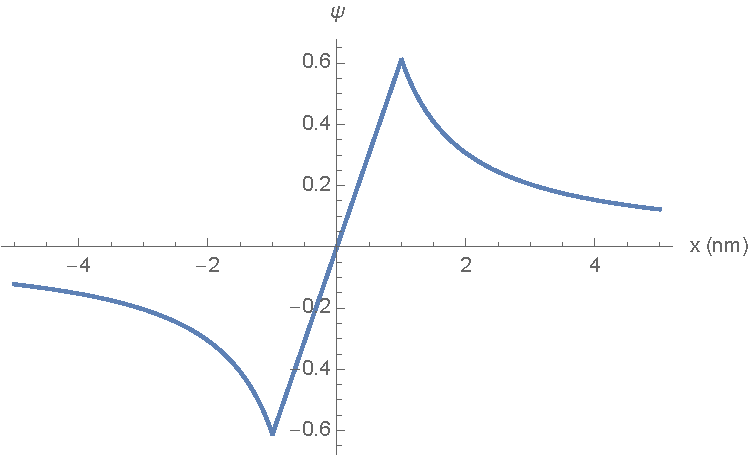
\includegraphics{psi-graph-raw}

        \item

        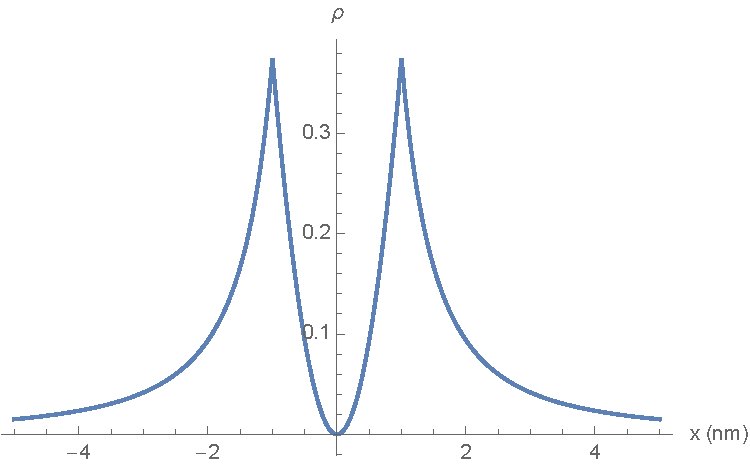
\includegraphics{pdf-graph}

        \item Using our known value for $c^2$,
        \begin{equation*}
            \rho = \int_{-1}^{1} |\psi(x)|^2 dx = \int_{-1}^{1} \frac{3}{8}x^2 = \frac{1}{4}
        \end{equation*}
        Therefore, $\SI{2.5e5}{}$ electrons will be found between $\pm\SI{1}{\nm}$.
    \end{enumerate}

    \item \begin{enumerate}
        \item Assuming $\alpha>0$,
        \begin{equation*}
            1 = 2b\int_{k_0}^{\infty} C^2e^{-2\alpha (k-k_0)} dk = \frac{bC^2}{\alpha} \implies b = \frac{\alpha}{C^2}
        \end{equation*}
        Since the Gaussian is symmetric, the total integral is twice the right half, as calculated above. Therefore,
        \begin{equation*}
            \psi(k) = \frac{\sqrt{\alpha}}{C} e^{-\alpha (k-k_0)^2}
        \end{equation*}


        \item The Fourier transform of $\psi(k)$ is given by
        \begin{equation*}
            \psi(x) = \frac{1}{\sqrt{2\pi}} \int_{-\infty}^{\infty} \psi(k) e^{ikt} dt =
            \left(\frac{\alpha}{2C}\right)^{\frac{1}{2}}e^{ik_0x}e^{-\frac{x^2}{4a}}
        \end{equation*}
        I know the constant here isn't right, sorry.

    \end{enumerate}

        \item \begin{enumerate}
            \item Conservation of energy is violated by $\Delta E = \SI{135}{\MeV/\clight^2}$. Because the pi meson has this mass, and appears out of nowhere, this is the amount of energy that must be spontaneously created.

            \item
            \begin{equation*}
                \Delta E \Delta t = \frac{\hbar}{2} \implies \Delta t = \frac{\hbar}{2\Delta E} = \frac{\SI{6.583e-16}{\joule\s}}{2(\SI{1.35e8}{\eV})} = \SI{2.44e-24}{\s}
            \end{equation*}

            \item If the pi meson travels near the speed of light, then the distance it can travel is about
            \begin{equation*}
                c(\Delta t) = (\SI{2.44e-24}{\s})(\SI{3e8}{\m/\s}) = \SI{7.31e-16}{\m}
            \end{equation*}
        \end{enumerate}

        \item Letting the angle of the incident proton be 0, the angle of the two scattered photons must be the same. Call this angle $\theta$. Then the angle between the photons, which we're trying to calculate, is given by $2\theta$. The momentum of each of the protons is also give by
        \begin{equation*}
            E^2 = (pc)^2 + (mc^2)^2 \implies p = \frac{\sqrt{E^2-(mc^2)^2}}{c}
        \end{equation*}
        We have that
        \begin{equation*}
            2 \frac{\sqrt{(E/2)^2-(mc^2)^2}}{c} \sin \theta = \frac{\sqrt{E^2-(mc^2)^2}}{c}
        \end{equation*}
        because the x-direction momentum must be conserved. This gives that
        \begin{equation*}
            \theta = \arcsin \left(\sqrt{\frac{E^2-(mc^2)^2}{E^2-(2mc^2)^2}}\right)
        \end{equation*}
        and so the angle between the two protons is
        \begin{equation*}
            2\theta = 2\arcsin \left(\sqrt{\frac{E^2-(mc^2)^2}{E^2-(2mc^2)^2}}\right)
        \end{equation*}
    \end{enumerate}


\end{document}
